% =============================================================================
% CAPÍTULO 4 — volta 1 (AGENTS.md §6): a forma da mudança decide o preço do silêncio.
%
% O fracasso que o abre, com número na mão: com o mesmo orçamento de um alarme por ano, o vigia
% vê um degrau em 7 dias, uma rampa em 69 e uma deriva em 149,5 — e nenhum ajuste de limiar
% encurta a distância. Encurtada a memória para um mês, as três formas chegam quase juntas.
%
% Medição: lab/experimentos/E03_formas.ipynb; a primeira figura (fig:formas) vem do E02, que
% mediu o orçamento. Figuras: figuras/E03_formas_*, figuras/E02_orcamento_3.
% =============================================================================

\chapter{A forma decide o preço}\label{cap:formas}

Falta uma peça, e ela é grande. O vigia do orçamento foi calibrado contra a cauda que se abre de
uma vez, e essa não é a única forma que a mudança tem. Cada forma cobra do mesmo silêncio um preço
diferente, e nenhum ajuste de limiar encurta a distância entre elas.

\section{Três formas de mudança}

Para medir isso sem depender de quais tombos o mercado ofereceu, usamos mundos em que a
mudança é posta de propósito, com data conhecida: séries de \numFormaMundoDias{} dias em que a
oscilação muda no dia \numFormaMudancaDia, e \numFormaRepeticoes{} repetições de cada forma.
São três.

\begin{itemize}[leftmargin=1.5em]
  \item o \textbf{degrau} --- a oscilação dobra de uma vez, e a partir dali fica assim;
  \item a \textbf{rampa} --- a oscilação cresce até dobrar ao longo de meses, de modo que
    nenhum dia isolado é extraordinário;
  \item a \textbf{deriva} --- a média se desloca um pouco a cada dia, sem que a oscilação mude
    em nada.
\end{itemize}

Mesma rotina, mesmo orçamento, e o resultado é uma diferença que nenhum ajuste de limiar
resolve.

No orçamento de \numFundoUmAnoAlarmesPorAno{} alarme por ano, o degrau foi visto em
\numFormaDegrauDias{} dias, a rampa em \numFormaRampaDias{} dias e a deriva em
\numFormaDerivaDias{} dias. Encurtando a memória para um mês, o orçamento fica falador
(\numFundoUmMesAlarmesPorAno{} alarme por ano) e as três formas chegam quase juntas: o degrau
em \numFormaCurtaDegrauDias{} dias, a rampa em \numFormaCurtaRampaDias{} e a deriva em
\numFormaCurtaDerivaDias.

\begin{figure}[htbp]
  \centering
  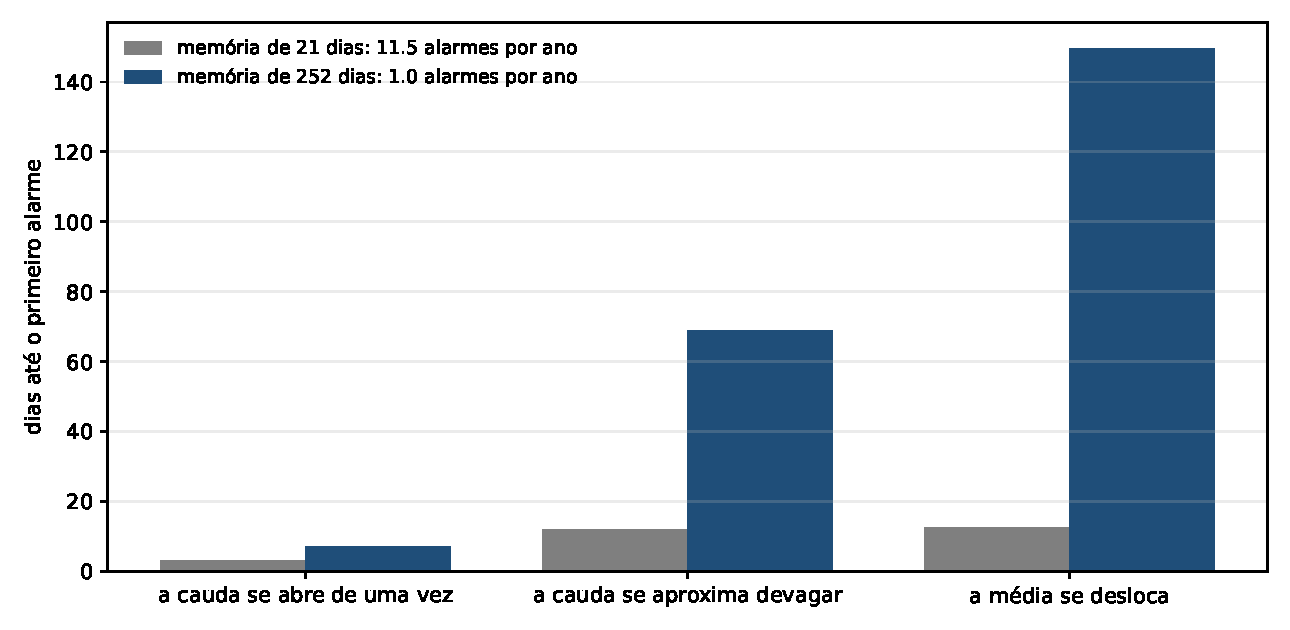
\includegraphics[width=\linewidth]{figuras/E02_orcamento_3.pdf}
  \caption{Dias até o primeiro alarme, por forma de mudança, em dois orçamentos: a memória de
    um mês, à esquerda de cada par, e a de um ano, à direita. O orçamento mais raro paga a
    diferença entre as formas.}
  \label{fig:formas}
\end{figure}

A leitura da figura é a leitura dos números. Com um orçamento raro, a mudança que o vigia vê
depressa é a cauda que se abre de uma vez, e a que ele vê devagar é a média que se desloca: a
mesma rotina, o mesmo silêncio prometido, e \numFormaDerivaDias{} dias contra
\numFormaDegrauDias. Com um orçamento falador, a distância entre as formas quase desaparece,
porque um alarme que soa a cada poucos dias não precisa esperar por nada.

Isso também diz o que a \cref{tab:troca} de fato mediu. A curva da troca foi desenhada com os
tombos do mercado, que são degraus; para uma deriva, a mesma curva estaria deslocada para a
direita, com o preço do silêncio pago em meses.

\section{O que a memória faz}

O corte é erguido com os dias que já passaram, e por isso ele acompanha o mundo. Poucos dias
depois de um degrau na oscilação, os piores dias da janela já são dias mudados, e o corte
desce junto com eles. Num mundo que passa a oscilar oito vezes mais, a contagem em
\numBlocoDias{} dias assenta em \numFormasContagemAdaptativaDegrau, onde a promessa admite
\numBlocoPrometido{} --- e o mundo segue oito vezes mais perigoso.

Vale comparar com o corte que não se mexe. Erguido uma vez e deixado parado, ele continua
medindo o mundo novo com a régua velha: a contagem assenta em \numFormasContagemFixaDegrau,
oito vezes a promessa, e não volta. No mundo parado os dois cortes dão a mesma coisa,
\numFormasContagemFixaParado{} contra \numFormasContagemParado, de modo que a diferença entre
eles não é de calibração. É de memória.

A promessa se sustenta porque a memória esquece. O mesmo movimento que restaura a taxa apaga
a mudança, e um vigia feito dessa taxa fica sem o que ver depois que a janela se renova: no
degrau de oito vezes isso custa \numFormasVigiaDegrauOitoDias{} dias, e na rampa do mesmo
tamanho final, \numFormasVigiaRampaOitoDias{} dias. A forma não muda o que aconteceu ao mundo. Muda o que sobra para o
vigia ver.

A deriva escapa aos dois cortes. Deslocar a média não mexe na oscilação, e a contagem sente
pouco: no corte fixo, uma deriva de \numFormasDerivaForteAnoPct\% ao ano leva a contagem de
\numFormasContagemFixaParado{} para \numFormasContagemFixaDeriva{}, quase nada, porque um
passo de dois décimos por cento contra um barulho de um por cento por dia mal move a cauda
esquerda.

Para essa forma existe outro instrumento, e ele mede outra coisa: a média da janela medida em
erros-padrão dela mesma (\texttt{centro.py}).
% aterramento: erro-padrao
O \textbf{erro-padrão} de uma média é o nome que a prática dá à barra: o desvio de um dia
dividido pela raiz do número de dias. Numa janela de dez dias em que cada dia oscila um por
cento, a média carrega um erro-padrão de um terço de um por cento, e é contra esse número que
ela mede a si mesma.
Ele vê a deriva forte em
\numFormasLeiForteDias{} dias, com \numFormasLeiForteNadaPct\% dos mundos sem alarme nenhum
no horizonte de \numFormasHorizonteDias{} dias. E é cego à escala: nos mundos de degrau e de
rampa ele não soa em quase oitenta por cento dos casos, porque dobrar a oscilação dobra o
erro-padrão da média e deixa a estatística onde estava.

O vigia da contagem vê as duas rampas, e vê mais depressa a maior: \numFormasVigiaRampaOitoDias{} dias
contra \numFormasVigiaRampaDoisDias. Fica sem ver nada dentro do horizonte em
\numFormasVigiaRampaOitoNadaPct\% dos mundos na rampa maior e \numFormasVigiaRampaDoisNadaPct\% na
menor. Contra isso vale o mundo parado: sem mudança nenhuma, o vigia leva
\numFormasVigiaParadoDias{} dias e fica sem alarme em \numFormasVigiaParadoNadaPct\% dos mundos, de modo
que as formas se leem contra esse chão.

A \cref{fig:instrumentos} põe os dois instrumentos lado a lado, e o que ela mostra é que
cada um vê uma forma e tropeça na outra.

\begin{figure}[htbp]
  \centering
  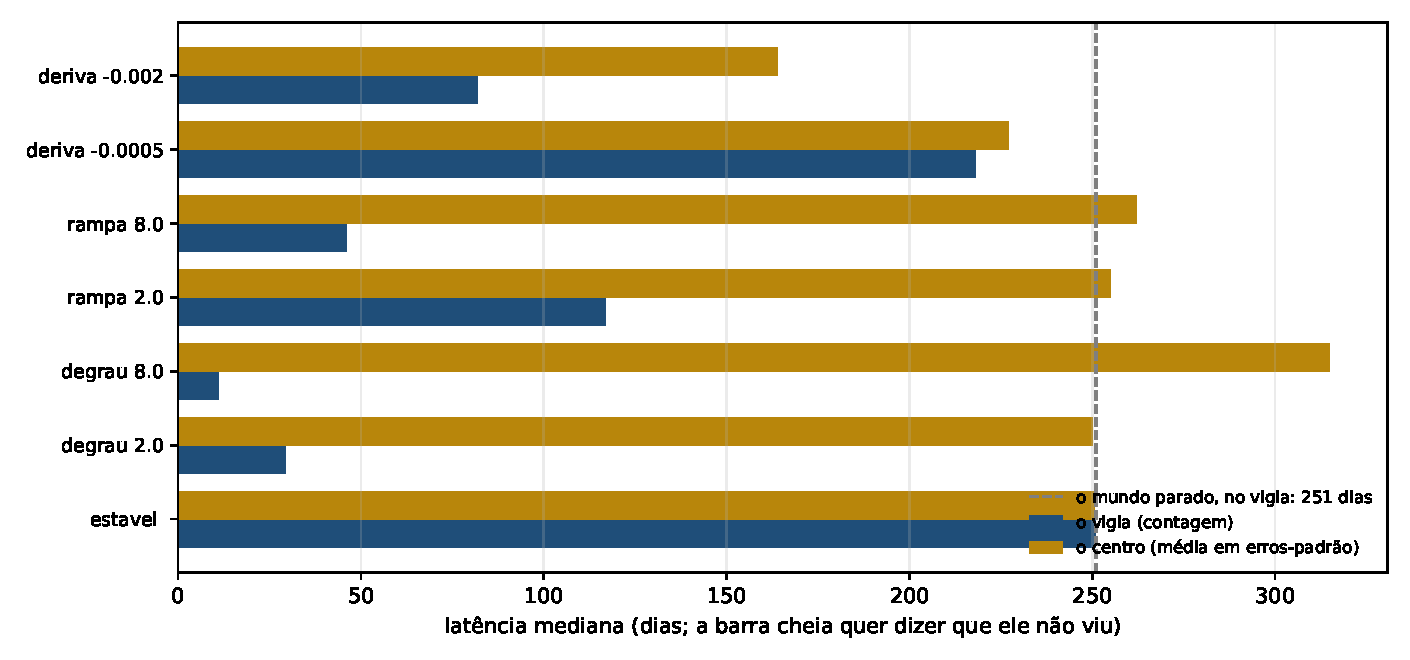
\includegraphics[width=\linewidth]{figuras/E03_formas_2.pdf}
  \caption{A latência mediana de cada instrumento, forma por forma: a contagem de rompimentos
    contra a média da janela em erros-padrão dela mesma. A linha tracejada é o que o mundo
    parado produz no primeiro deles, e duas barras que terminam no mesmo lugar merecem cuidado: o
    mundo parado não é uma forma de mudança, e é ele que reaparece em toda forma.}
  \label{fig:instrumentos}
\end{figure}

% aterramento: latencia
% aterramento: sigma
A demora dele se paga em memória, e a conta fecha em duas linhas. Chamo de \textbf{latência} os
dias que um instrumento leva para dar o alarme, contados do dia em que o mundo mudou: é o atraso
dele, na mesma unidade das tabelas. O barulho de um dia --- o tamanho típico do que ele anda por
conta própria --- escreve-se $\sigma$, e o passo com que a média se desloca escreve-se $p$; os
dois na mesma unidade do dado. Uma regra
de $L$ erros-padrão vê uma deriva de passo $p$ contra um barulho $\sigma$ quando a janela tem
$(L\sigma/p)^2$ dias --- e a latência mínima é esse mesmo número, porque o instrumento
precisa dos dias antes de poder julgá-los. Com um ano de memória, a regra enxerga a deriva
que o barulho esconde por um fator de $\sqrt{\numCorteJanela}$; com catorze anos, uma quatro
vezes menor. Para a deriva de \numFormasDerivaLeveAnoPct\% ao ano, a memória
exigida é de \numFormasMemoriaDerivaLeve{} dias: no horizonte de \numFormasHorizonteDias{}
dias nenhum mundo alarmou, e o motivo não é cegueira. É que a memória que ele pede é maior do
que o tempo que se esperou.

\begin{figure}[htbp]
  \centering
  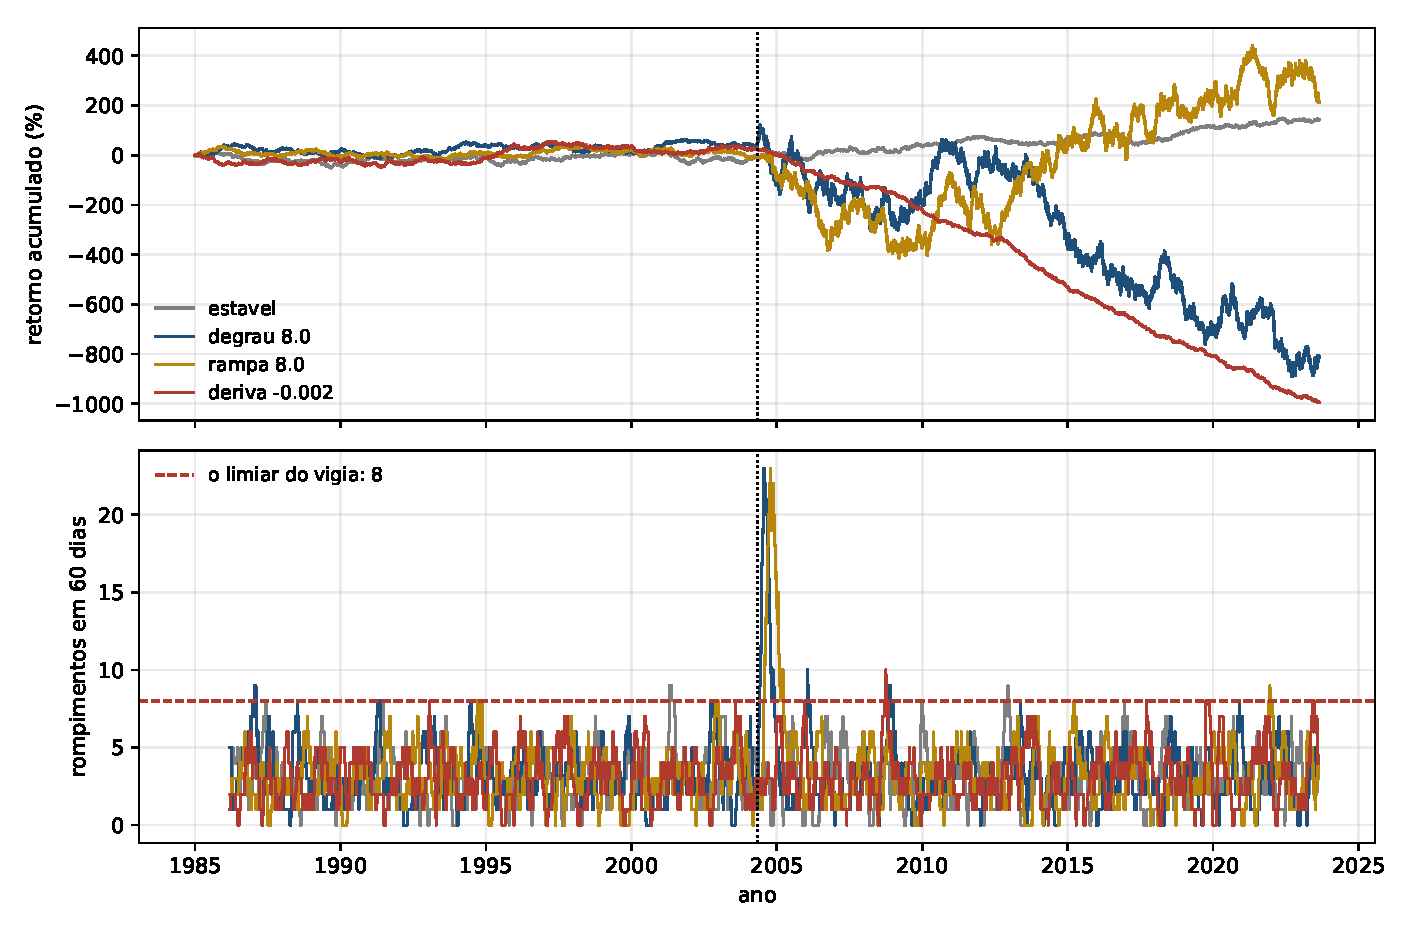
\includegraphics[width=\linewidth]{figuras/E03_formas_1.pdf}
  \caption{Três mundos de quarenta anos com a mudança no meio (linha pontilhada), e o mundo parado
    como chão. Em cima, o retorno acumulado; embaixo, os rompimentos do corte em
    \numBlocoDias{} dias, com o limiar do vigia. A deriva é o único mundo que cai, e é o
    único em que a contagem não sobe.}
  \label{fig:memoria}
\end{figure}

\section{O que fica}

Fica a forma, e ela é um preço: o mesmo silêncio declarado custa \numFormaDegrauDias{} dias para
uma cauda que se abre de uma vez e \numFormaDerivaDias{} dias para uma média que se desloca. Fica
com ela o que a memória faz, que é a outra metade da conta: o corte acompanha o mundo porque
esquece, e o mesmo movimento que restaura a taxa apaga a mudança.

E fica o segundo instrumento, que vê a forma que a contagem não vê. A contagem de rompimentos vê
o degrau e a rampa e é cega à deriva; a média da janela medida em erros-padrão dela mesma vê a
deriva e é cega à escala. Cada um vê uma forma e tropeça na outra.

As outras duas formas que o mundo tem não aparecem em nenhum dos dois. Duas séries podem
passar a cair juntas sem que nenhuma das duas mude de tamanho, e o calendário pode passar a
juntar as coisas ruins na mesma semana sem que nenhum dia fique maior: não há dia para romper
a linha, e não há limiar que veja. Medir essas formas exige um terceiro instrumento, e é a
pergunta seguinte.
